\section{Preliminary Results}
\subsection{Experimental setup}
Figure \ref{fig:experiment_schematics} presents the schematic of the experimental setup. The sample is held in a cryostat  at a temperature of 5K. The PL is collected using an objective lens with a numerical aperture of 0.85. The same objective also focuses the exciting lasers into the sample. We used a tunable, $76\,\rm MHz$ pulsed laser for the lifetime measurement and a CW, $632.8\,\rm nm$ HeNe laser, to perform the correlation measurements. \\
	\begin{figure}[H]
		\centering
		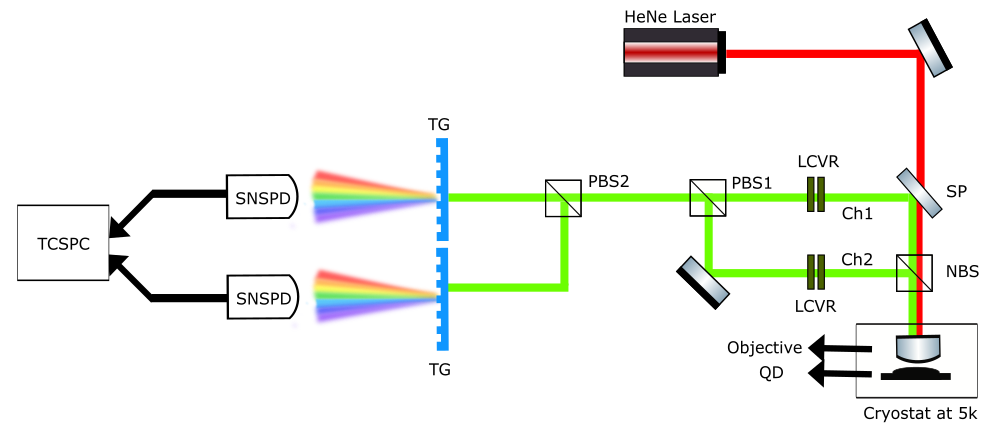
\includegraphics[scale=0.60]{figures/Experiment_schematics.png}
		\caption{Schematics of the measurement setup.}
		\label{fig:experiment_schematics}
	\end{figure}
The PL collected from the dot is split into two channels using a non-polarizing beam splitter (BS), wherein one of the channels, a short pass filter (LP), is used for transmitting the laser while reflecting the PL.\\
In both channels, the PL passes through a liquid crystal variable retarder (LCVR), which projects its polarization onto the axis of the first polarized beam splitter (PBS), where both channels recombine such as the H(V) polarization of the first(second) channel combine with the V(H) polarization from the second(first) channel and vice versa. Finally, the PL reaches the transmission grating (TG), where the PL is dispersed, and only photons with specific energy reach the superconducting nanowire single photon detector (SNSPD). The signal emitted from the detector is sent to a time-correlated single photon counter (TCSPC) that registers the time information about the events and saves it for analysis. 
\subsection{Photoluminescence Spectroscopy}
In photoluminescence (PL) spectroscopy, emitted light from the QD sample is spectrally dispersed in a transmission grating. Several optically-active transitions of the QD system can be studied using a CCD camera  as seen in figure \ref{fig:Spectrum_HV}. The excitation laser power can be varied, changing the number of carrier pairs that occupy the dot. The QD is most likely occupied by single neutral or charged excitons at low excitation power. At higher excitation power, biexciton and states with similar configurations become visible. Measuring the spectrum as a function of power can yield some of the information necessary to identify the observed transitions. Changing the illumination source, or varying the sample temperature, results in the appearance of emission lines corresponding to charged states and enables examination of QD charging processes.\\
The PL spectrum can also be measured with variable polarization, and these measurements also provide information about the type of optical transitions observed. For example, the neutral excitonic and biexcitonic optical transitions display a fine structure HV-polarized doublet. Charged excitonic transitions are, on the other hand, unpolarized but have strong polarization memory [60]. Studies of the polarization behavior of spectral lines can aid in the identification of the transitions [3, 12, 19, 48, 20]
\begin{figure}[H]
		\centering
		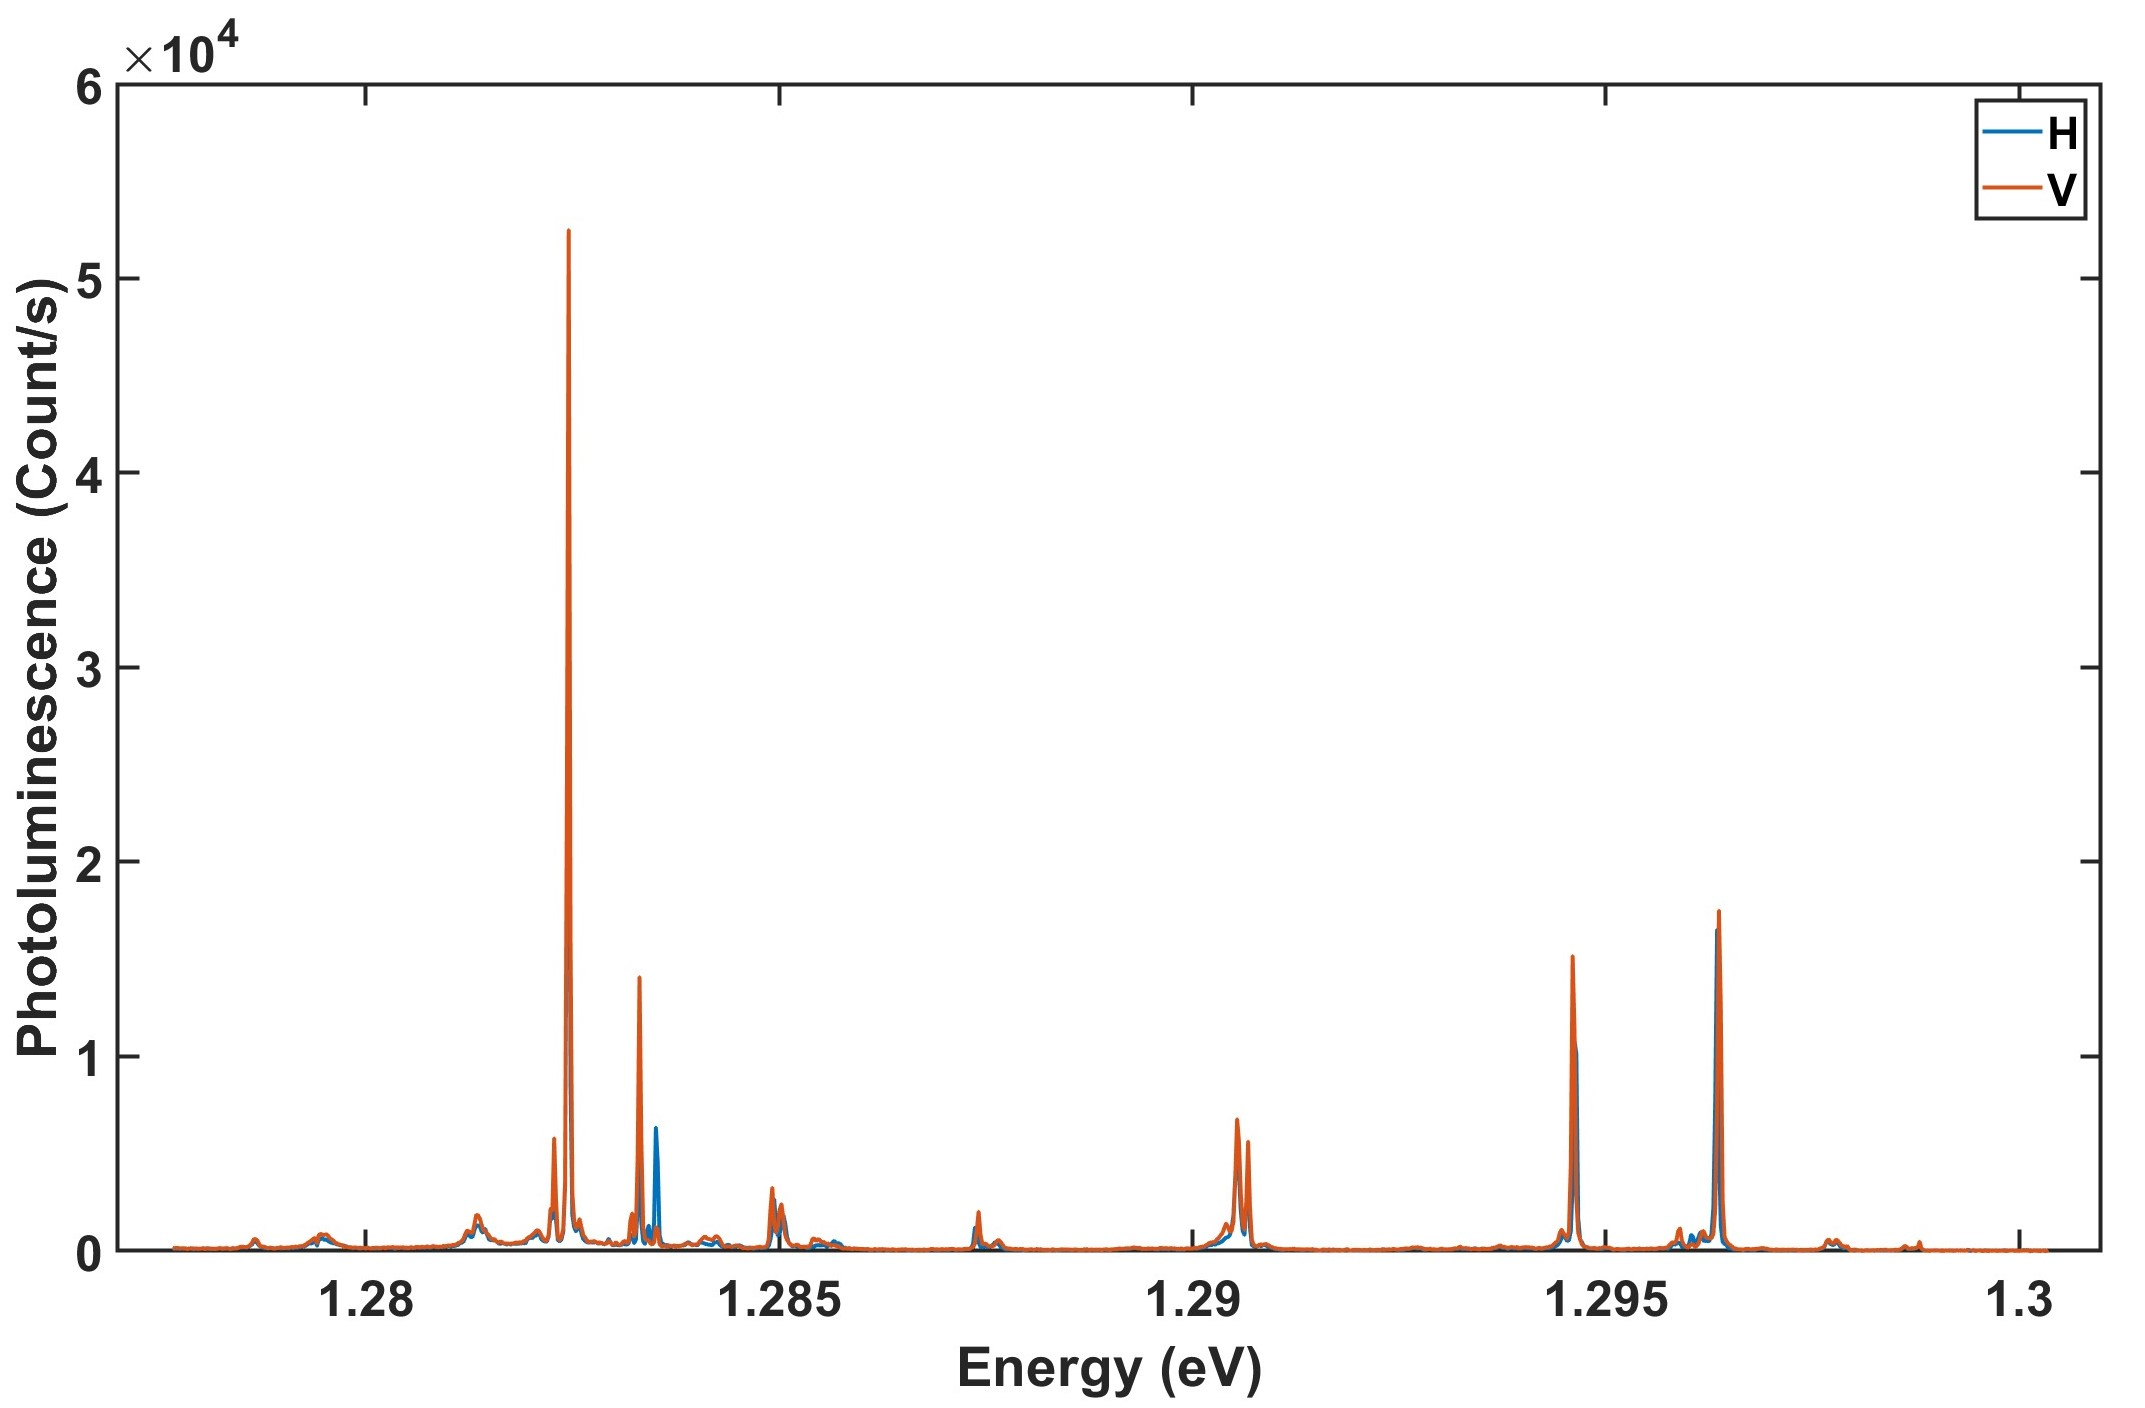
\includegraphics[scale=0.27]{figures/Spectrum.jpg}
		\caption{Polarization-dependent photoluminescence spectra from a single quantum dot in a microcavity under non-resonant excitation using HeNe laser for horizontal (H) and vertical (V) polarization.}
		\label{fig:Spectrum_HV}
	\end{figure}
\subsection{Exciton-biexciton cascade under CW excitation}
The second-order intensity correlation function between the emission lines of the biexciton-exciton can be described as:
\begin{equation} \label{second_order_correlations}
\begin{aligned} 
        g_2(\tau) = \frac{\langle I_{XX}(t) \cdot<I_{X}(t+\tau) \rangle}{\langle I_{XX}(t)\rangle \cdot\langle I_{X}(t)\rangle}
\end{aligned}
\end{equation}
where $I_{XX}(t)$ ($I_X(t)$) is the emission intensity of the biexciton (exciton), averaged over the time t.
\begin{figure}[H]
	\centering
	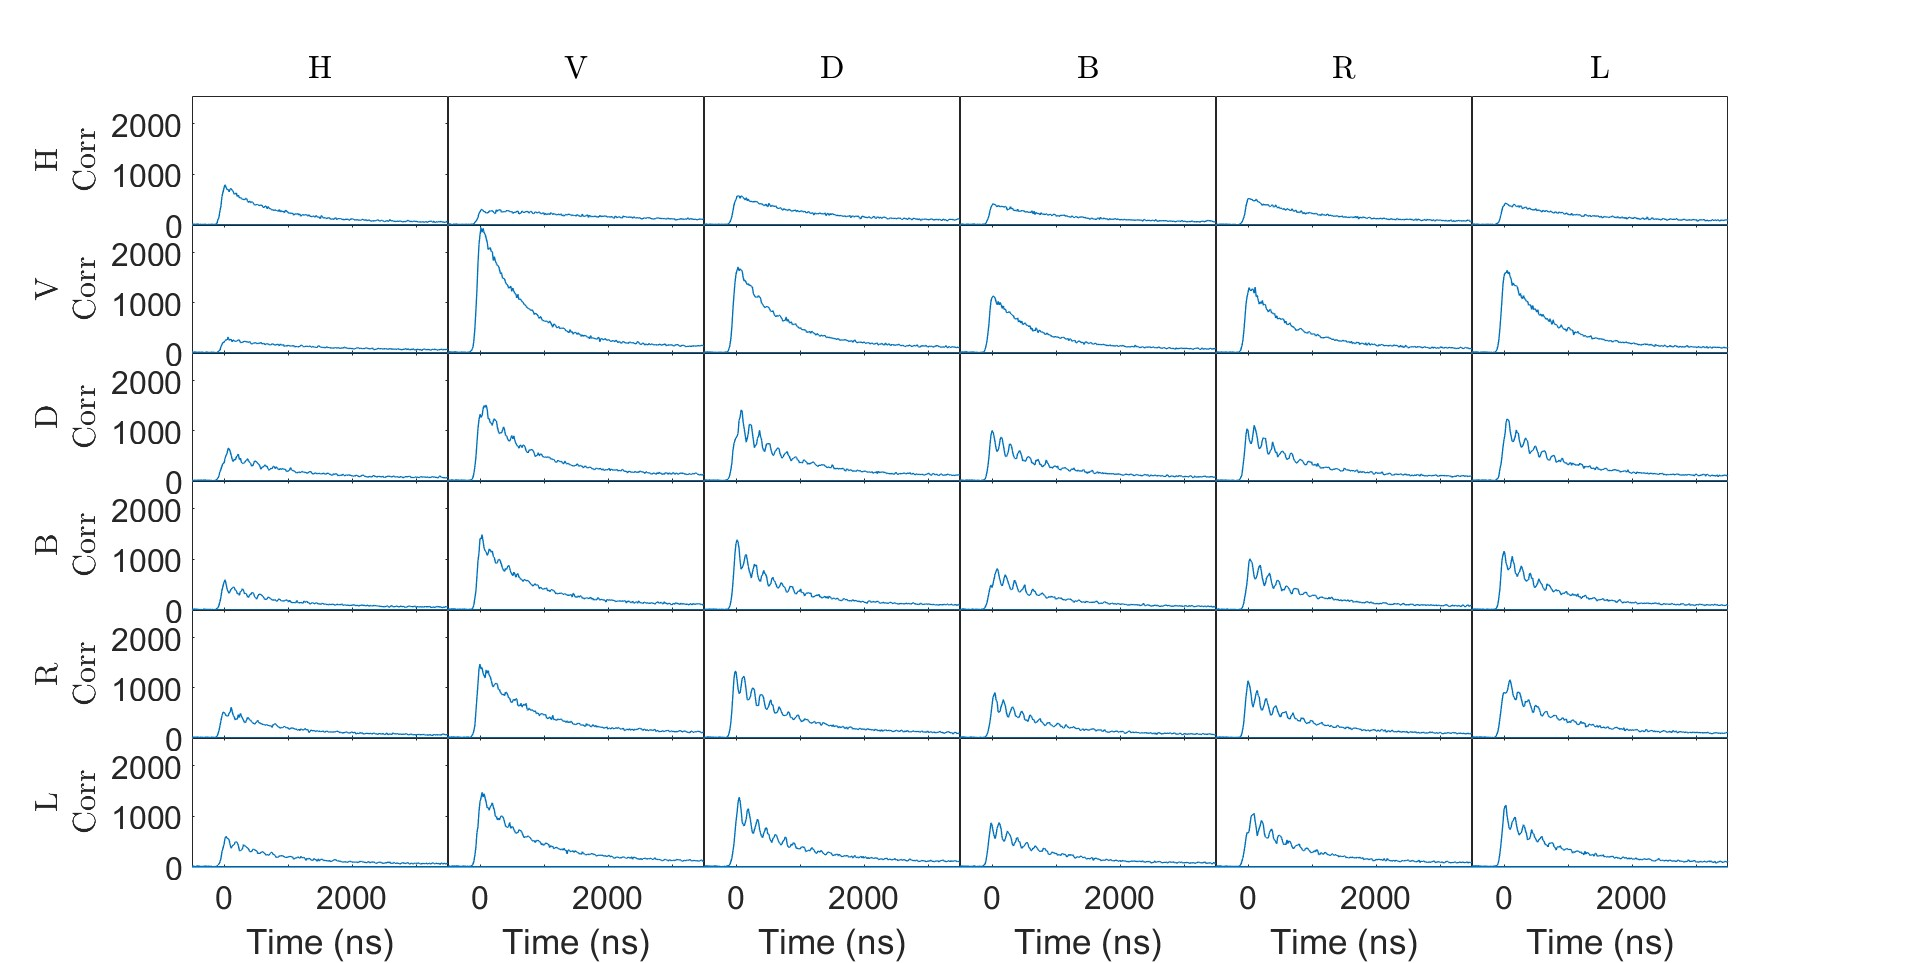
\includegraphics[scale=0.24]{figures/XX_X_Correlations.jpg}
	\caption{ The second-order correlations of the biexciton-exciton radiative cascade., where each row (column) represents a biexciton (exciton) photon polarization (H,V,D,B,R,L).}
	\label{fig:XX_X_Correlations}
\end{figure}
\subsection{Exciton-biexciton cascade under pulsed excitation}
\subsection{Mach-Zehnder Interferometer}
The Mach-Zehnder interferometer consists of a light source that produces a coherent beam of light, which is then split into two separate paths by a beam splitter. Each path contains a series of mirrors reflecting the light back toward the beam splitter. The two reflected beams are recombined at the beam splitter and directed toward a detector.\\
When the two beams are in phase, they will constructively interfere and produce a bright spot on the detector. When they are out of phase, they will destructively interfere and produce a dark spot. By varying the path length of one of the arms of the interferometer, the relative phase between the two beams can be changed, causing the interference pattern to shift from bright to dark or vice versa.
\subsubsection{Schematic}
The basic description of the interferometer is presented in figure \ref{fig:Mach_zhender}. The photons emitted from the quantum dot (blue) are split using a polarized beam splitter (PBS), where the vertical component is reflected. Then couples to polarization maintaining (PM) fiber attached to the phase modulator controlled using an arbitrary wavefunction generator. In contrast, the horizontal component is transmitted and then couples to another PM fiber. Afterward, The vertical and horizontal components recombine at the interferometer's output using a second PBS. The two paths must be the same length for recombining the two components.
\begin{figure}[H]
		\centering
		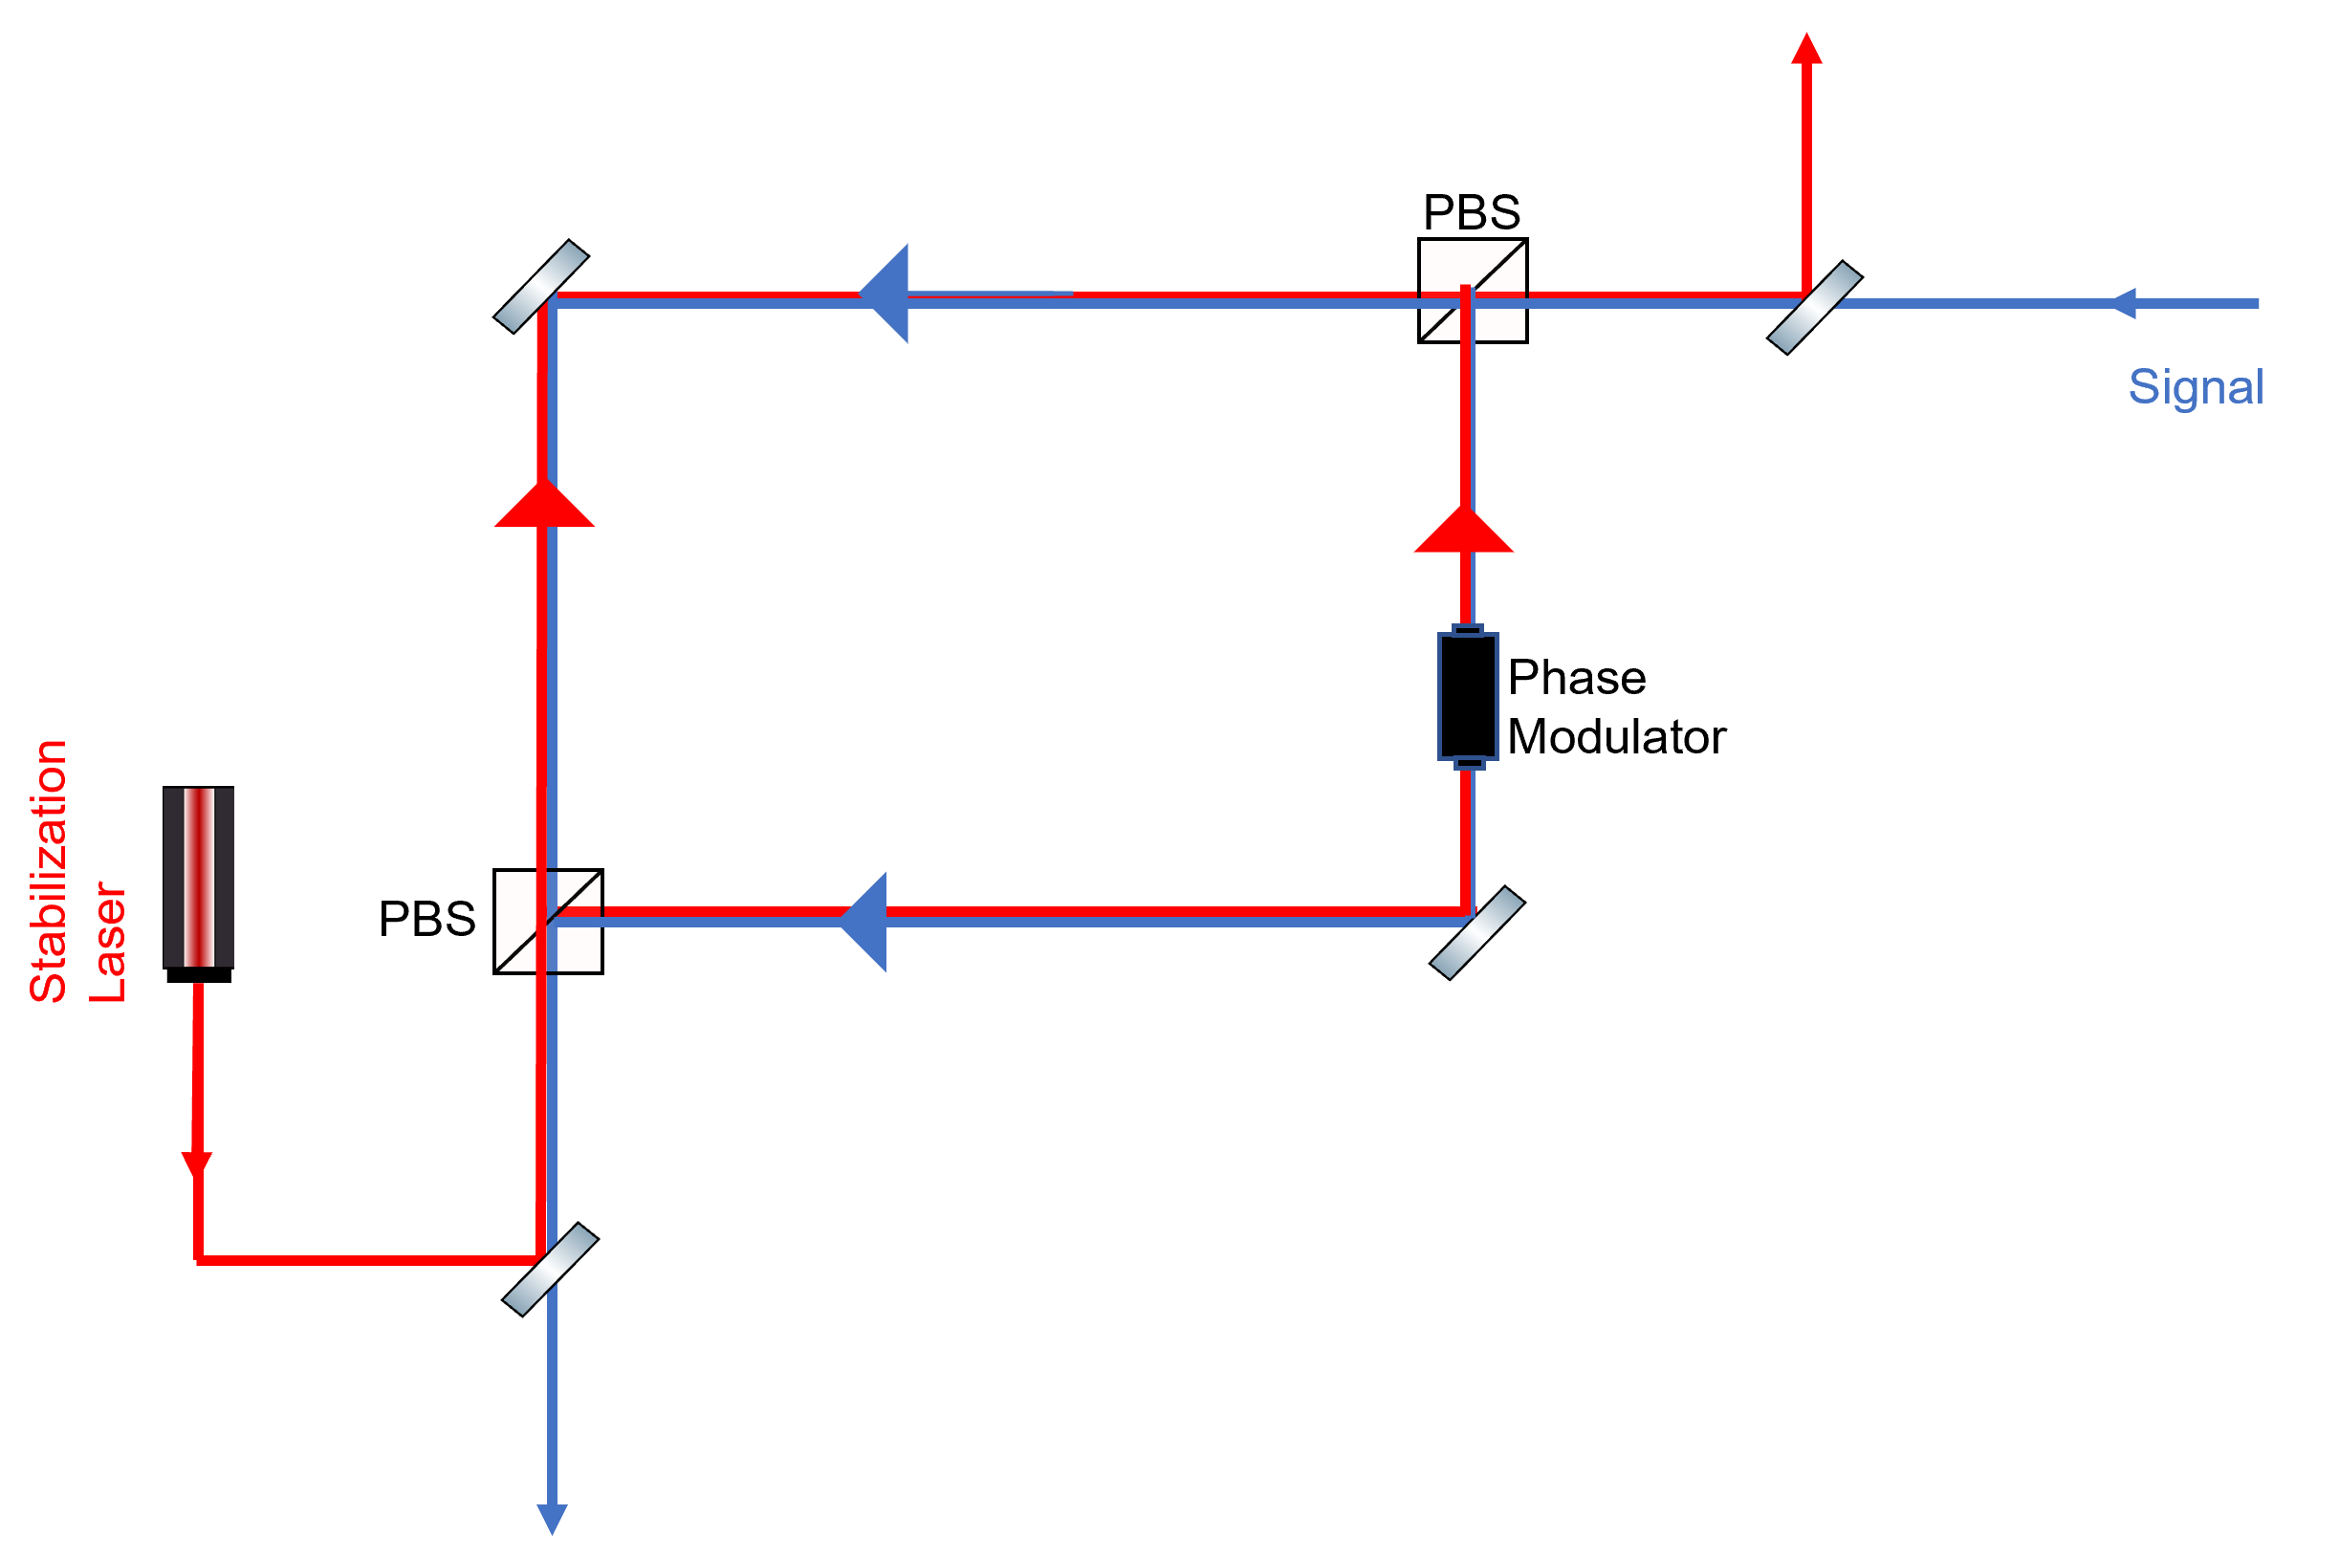
\includegraphics[scale=0.70]{figures/Mach_Zhender Interferometer.png}
		\caption{Schematics of the Mach-Zehnder Interferometer.The path of the signal from the quantum dot in blue and the laser for the active stabilization in red}
		\label{fig:Mach_zhender}
	\end{figure}
 The introduction of fibers into the Mach-Zehnder introduces phase instability to it. This can be due to temperature variations, vibrations, or airflow around the fibers. While these factors can be minimized or eliminated, A completely stable interferometer remains difficult; Therefore, we must construct an active stabilization method using a feedback loop for a more stable interferometer.\\
 The feedback loop is constructed using a $4^{\circ}$ wedge mounted on a slider that can be displaced using a piezo motor. This wedge is added to one of the arms of the interferometer, which allows us to adjust the path length. Next, we introduce a laser signal to the interferometer as seen in figure \ref{fig:Mach_zhender} in red. This laser is combined and separated from the quantum dot signal using Neutral Density (ND) filters or dichroic mirrors at the in and out ports, propagating in the opposite direction from the signal emitted from the quantum dot. \\
 After the signal from the laser passes through the interferometer, we collect it using a detector which allows us to observe the stability of the interferometer. The signal will drift with time, representing the  phase difference between the two arms, where the minimum and maximum counts observed represent destructive and constructive interference. To stabilize the interferometer, We move the piezo motor in 0.3 intervals based on the count measured at the detector until we achieve destructive interference.
\subsubsection{Measurements of stability}
To assess the stabilization quality, We measure the laser signal for a period of time for the case with active stabilization and one without. The data is plotted in a histogram as shown in figure \ref{fig:stablization_histogram}.
\begin{figure}[H]
	\centering
	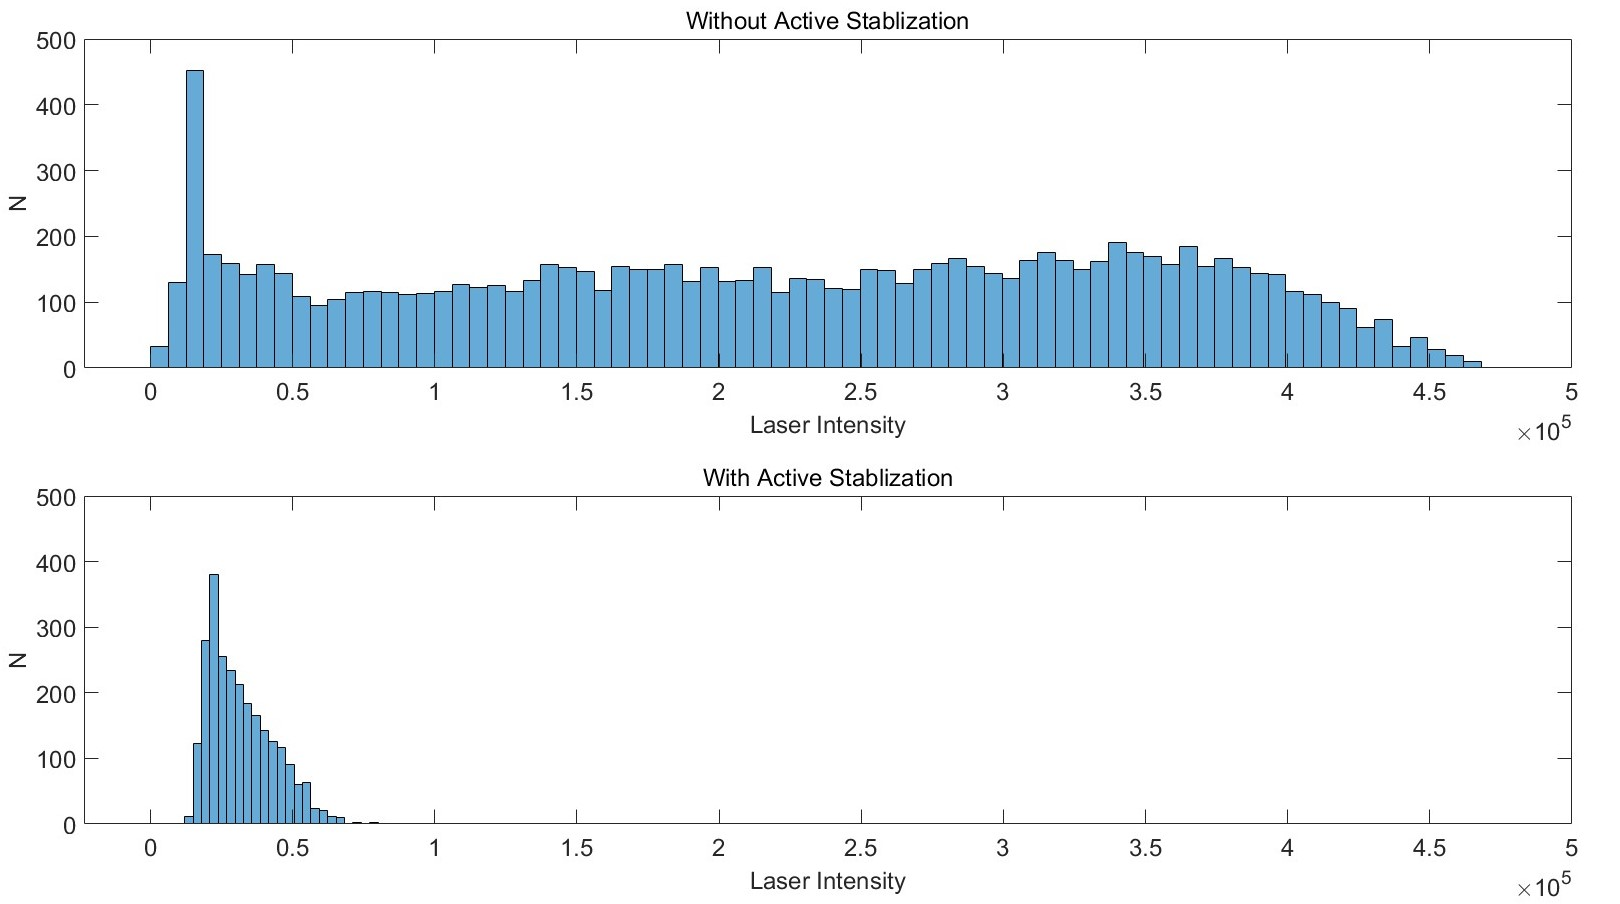
\includegraphics[scale=0.32]{figures/StablizationHistogram.jpg}
	\caption{}
	\label{fig:stablization_histogram}
\end{figure}
First, the stability of the interferometer is tested without the correction feedback. The data collected is presented in figure \ref{fig:stablization_histogram}a. as seen, the count from the detector is evenly distributed at all intervals. In active stabilization, the count is distributed around the minimum.